\chapter{Obsah CD}
Praktická část práce je uložena na CD. Obsah CD a jeho popis:
\begin{itemize}
\item \texttt{doc} - dokumentace k práci \texttt{IBP\_MsPacman\_Blozonova.pdf}
\item \texttt{src} - zdrojové kódy frameworku (včetně složky \texttt{layouts} s mapami pro \texttt{pacman.py}) s implementacemi agentů a vektoru vlastností v souborech:
\begin{itemize}
\item \texttt{multiAgents.py} - implementace chování základních agentů
\item \texttt{valueiterationAgents.py} - implementace chování \texttt{valueiterationAgent}
\item \texttt{qlearningAgents.py} - implementace chování \texttt{QLearningAgent}, \texttt{PacmanQAgent} a \texttt{ApproximateQAgent}
\item \texttt{featureExtractors.py} - implementace vektoru vlastností \texttt{BetterExtractor}.
\end{itemize}
\end{itemize}

\chapter{Manuál}
\label{priloha:manual}
\section{Ms. Pacman demo (\texttt{pacman.py})}
\label{priloha:manualp}
Pro demo Ms. Pacman byly používány základní parametry:
\begin{itemize}
\item \texttt{-h} pro výpis celé nápovědy a všech možných parametrů
\item \texttt{-m} manuální režim (vyzkoušení grafického rozhraní dema)
\item \texttt{--frameTime 0} bez animace
\item \texttt{-q} minimalistický režim bez grafického rozhraní
\item \texttt{-t} textový režim bez grafického rozhraní 
\item \texttt{-f} fixed random seed (pro fixní modelaci náhodnosti scénářů)
\item \texttt{-z 0.7} míra zvětšení grafiky (\textit{zoom})
\item \texttt{-n 2010} počet epizod celkově
\item \texttt{-x 2000} počet tréninkových epizod
\item \texttt{-l smallClassic} druh mapy (ze složky \texttt{src/layouts}) - např. \texttt{smallClassic}, \newline \texttt{mediumClassic}, \texttt{minimaxClassic}, \texttt{openClassic},...
\item \texttt{-p ApproximateQAgent} druh agenta - např. \texttt{ReflexAgent}, \texttt{ExpectimaxAgent}, \newline \texttt{PacmanQAgent}, \texttt{ApproximateQAgent},...
\item \texttt{-a depth=3,alpha=0.7,epsilon=0.5,discount=0.9} agentovy další parametry,\newline např. hloubka \textbf{depth}, gamma \textbf{discount}
\end{itemize}
\subsection{Příklady použití}
\texttt{ReflexAgent}, 2 nepřátelé, defaultní mapa
\begin{lstlisting}[language=Python,texcl=true]
python pacman.py -p ReflexAgent -k 2
\end{lstlisting}
\texttt{ExpectimaxAgent}, 5 her se základním výpisem bez GUI, hloubka 3
\begin{lstlisting}[language=Python,texcl=true]
python pacman.py -p ExpectimaxAgent -l smallClassic -a depth=3,
-n 5 -q
\end{lstlisting}
\texttt{PacmanQAgent}, 2000 epizod tréninku, 10 zobrazených epizod provádění optimální strategie, na mapě \texttt{smallGrid}
\begin{lstlisting}[language=Python,texcl=true]
python pacman.py -p PacmanQAgent -x 2000 -n 2010 -l smallGrid
\end{lstlisting}
\texttt{PacmanQAgent}, 10 epizod tréninku na mapě \texttt{smallGrid}
\begin{lstlisting}[language=Python,texcl=true]
python pacman.py -p PacmanQAgent -n 10 -l smallGrid -a
numTraining=10
\end{lstlisting}
\texttt{ApproximateQAgent} 100 epizod z nichž 90 trénink (10 zobrazených epizod provádění optimální strategie), na mapě \texttt{mediumGrid}, použitý lepší Extractor vlastností
\begin{lstlisting}[language=Python,texcl=true]
python pacman.py -p ApproximateQAgent -a extractor=BetterExtractor
-n 100 -x 90 -l mediumClassic
\end{lstlisting}

\section{Gridworld problémy (\texttt{gridworld.py})}
\label{priloha:manualg}
Pro vizualizaci hodnot pokročilých agentů - především agenta \texttt{ValueIterationAgent} byly používány základní parametry včetně příkladů hodnot:
\begin{itemize}
\item \texttt{-h} pro výpis celé nápovědy a všech možných parametrů
\item \texttt{-m} manuální režim (pro řízení agentova chování při epizodách)
\item \texttt{-q} minimalistický režim bez grafického rozhraní
\item \texttt{-t} textový režim bez grafického rozhraní
\item \texttt{-w 120} pixelový rozměr políčka mřížky (lepší nastavit například na 120 px, jinak je mřížka příliš velká)
\item \texttt{-k 10} počet epizod
\item \texttt{-i 100} počet iterací V-hodnot
\item \texttt{-v} zobrazení hodnot po každé iteraci
\item \texttt{-g BookGrid} druh gridworld problému - např. \texttt{BookGrid}, \texttt{BridgeGrid}, \texttt{DiscountGrid}
\item \texttt{-a value} druh agenta - \texttt{value} pro Value Iteration, \texttt{q} pro Q-Learning
\item \texttt{-d 0.8} velikost koeficientu gamma
\item \texttt{-r 0.9} \textbf{livingReward}, odměna přechodu ze stavu do neterminálního následníka
\item \texttt{-n 0.2} \textbf{noise}, pravděpodobnost přechodu 
\item \texttt{-e 0.5} \textbf{epsilon} (epsilon-greedy), náhodnost akcí při tréninku
\item \texttt{-l 0.7} \textbf{alpha} (learning rate), rychlost TD učení
\end{itemize}
\subsection{Příklady použití}
\texttt{ValueIterationAgent}, defaultní mapa, 100 iterací, 10 epizod celkem
\begin{lstlisting}[language=Python,texcl=true]
python gridworld.py -a value -i 100 -k 10
\end{lstlisting}
\texttt{ValueIterationAgent}, typ gridworld problému \texttt{DiscountGrid}, 5 iterací, 10 epizod (výchozí)
\begin{lstlisting}[language=Python,texcl=true]
python gridworld.py -a value -i 5 -g DiscountGrid
\end{lstlisting}
\texttt{ValueIterationAgent}, překonání gridworld problému \texttt{BridgeGrid}, 1000 iterací, \texttt{gamma} = 0.9, \texttt{noise} =  0.1
\begin{lstlisting}[language=Python,texcl=true]
python gridworld.py -a value -i 1000 -g BridgeGrid --discount 0.9
--noise 0.01
\end{lstlisting}
\texttt{QLearningAgent}, 5 epizod celkově, manuálně
\begin{lstlisting}[language=Python,texcl=true]
python gridworld.py -a q -k 5 -m
\end{lstlisting}
\texttt{QLearningAgent}, 20 epizod na problému \texttt{DiscountGrid}, \texttt{alpha} = 0.8, \texttt{epsilon} = 0.5
\begin{lstlisting}[language=Python,texcl=true]
python gridworld.py -a q -k 20 -g DiscountGrid -l 0.8
--epsilon 0.5
\end{lstlisting}

\chapter{Přidatné obrázky k experimentům}
\label{pril:experobr}
\begin{figure}[!htbp]
\begin{center}
  \scalebox{0.35}{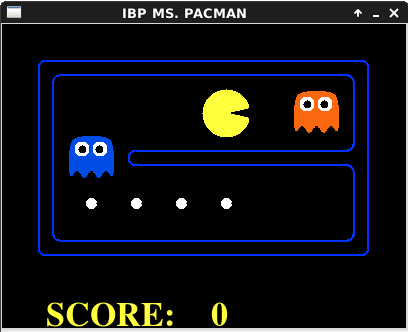
\includegraphics{img/trappedClassic.png}}
  \caption{Screenshot mapy \texttt{trappedClassic}.}
  \label{img:trapped}
\end{center}
\end{figure}

\begin{figure}[!htbp]
\begin{center}
  \scalebox{0.35}{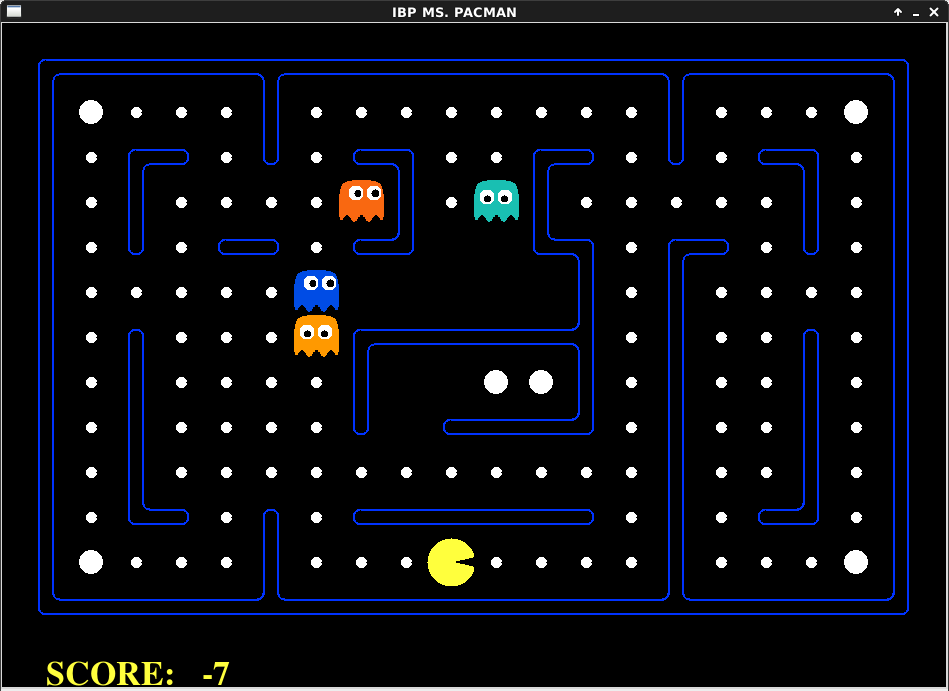
\includegraphics{img/trickyClassic.png}}
  \caption{Screenshot zatěžkávací mapy \texttt{trickyClassic}.}
  \label{img:tricky}
\end{center}
\end{figure}

\label{pril:experobr}
\begin{figure}[!htbp]
\begin{center}
  \scalebox{0.4}{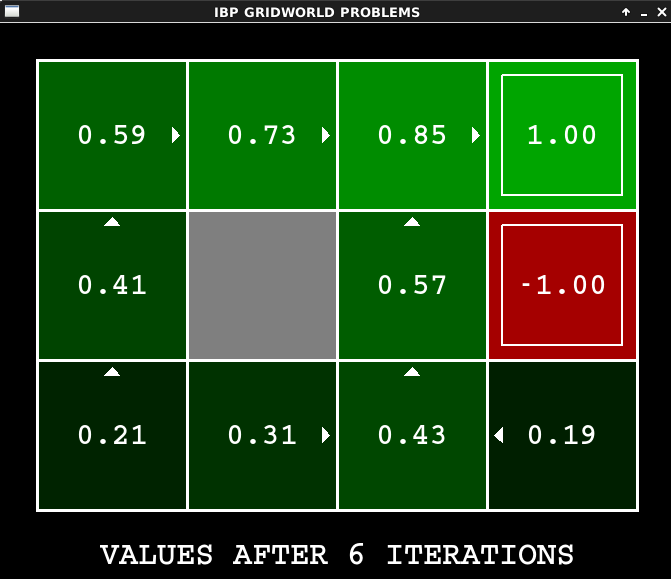
\includegraphics{img/valiter6.png}}
  \caption{Screenshot 6 iterací Value Iteration pro gridworld problém \texttt{BookGrid}.}
  \label{img:valiter6}
\end{center}
\end{figure}

\begin{figure}[!htbp]
\begin{center}
  \scalebox{0.35}{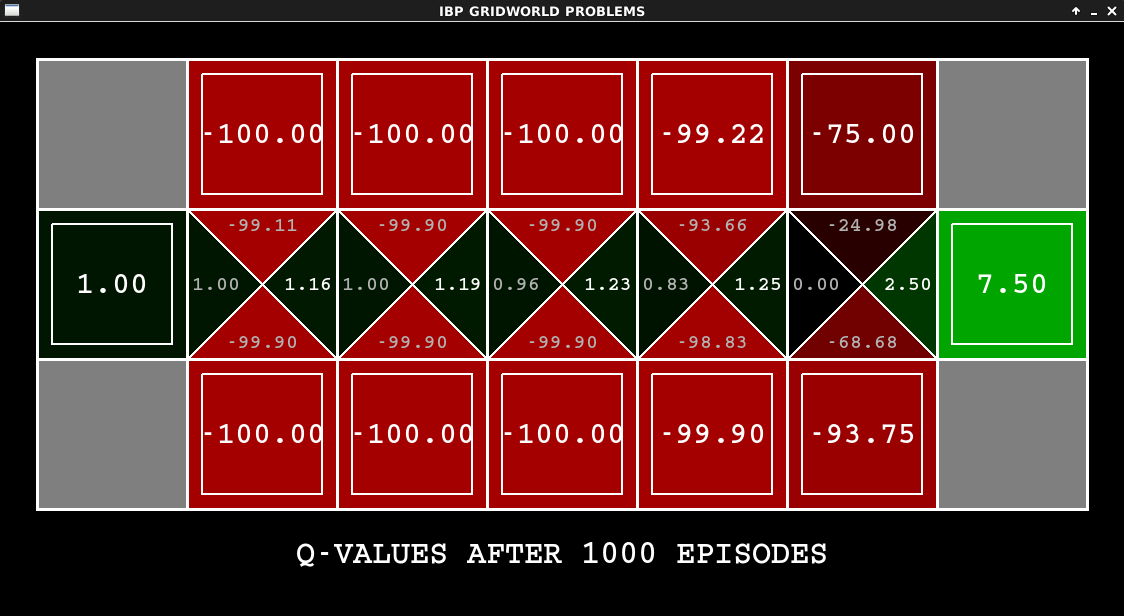
\includegraphics{img/bridgeq.png}}
  \caption{Screenshot Q-hodnot agenta \texttt{QLearningAgent} po 1000 epizodách na \texttt{BridgeGrid}.}
  \label{img:bridgeq}
\end{center}
\end{figure}

\begin{figure}[!htbp]
\begin{center}
  \scalebox{0.35}{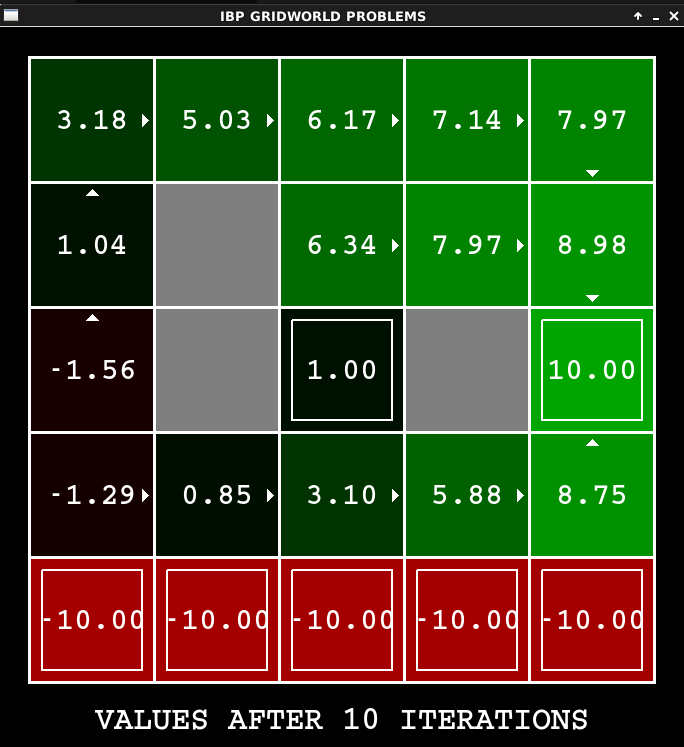
\includegraphics{img/discountPolicy.png}}
  \caption{Screenshot V-hodnot agenta \texttt{ValueIterationAgent} na \texttt{DiscountGrid}. Agent zde preferuje vzdálenější terminální uzel kratší cestou, ačkoliv riskuje pád z útesu.}
  \label{img:discountPolicy}
\end{center}
\end{figure}

\begin{figure}[!htbp]
\begin{center}
  \scalebox{0.35}{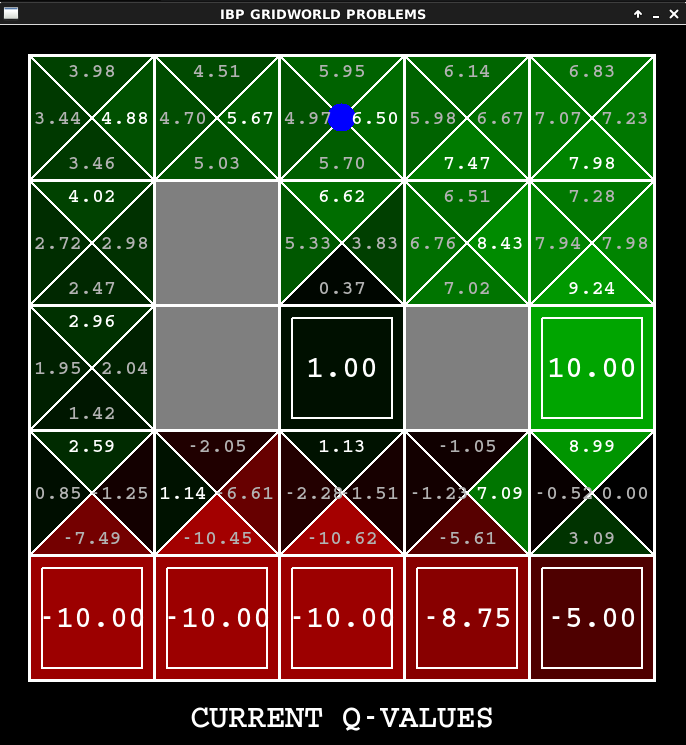
\includegraphics{img/discountPolicyQ.png}}
  \caption{Screenshot průběžných Q-hodnot agenta \texttt{QLearningnAgent} na \texttt{DiscountGrid}. Agent zde preferuje vzdálenější terminální uzel a delší bezpečnější cestu.}
  \label{img:discountPolicyQ}
\end{center}
\end{figure}

%\chapter{Konfigrační soubor}
%\chapter{RelaxNG Schéma konfiguračního soboru}
%\chapter{Plakat}

